\chapter{Portfolio Management}
Portfolio is basically a collection of (risky or risk free) assets. The general goal of a rational investor is to minimize the risk and maximize the profit. But high returns are generally associated with high risks.
\section{Risk and Return}
Warren Edward Buffett is an American investor and CEO of Berkshire Hathaway. He says -
\begin{itemize}
    \item Don't put all your eggs in one basket.
    \item Diversification may preserve wealth, but concentration builds wealth.
\end{itemize}
These two statements at the first glance seem to be contradictory but the first one says to minimize risk and the second one says to maximize returns.
\subsection{Expected Return}
 Suppose we invest $S(0)$ amount in some stock at time $t=0$, at time $t=T$ the price $S(T)$ is unknown and hence assumed to be a random variable. $S(T) : \Omega \rightarrow [0,+\infty]$ on a probability space $\Omega$.
 The return will be
 \begin{equation}
     K = \frac{S(T)-S(0)}{S(0)}
 \end{equation}
 This $K$ is a random variable with expected value $\mathbb{E}(K)=\mu_{K}=\mu$.
 By the linearity of mathematical expectation 
\begin{equation}
    \mathbb{E}(K)=\frac{\mathbb{E}(S(T))-S(0)}{S(0)}
\end{equation}
Hence $$S(T)=S(0)(1+K)$$ $$\mathbb{E}(S(T))=S(0)(1+\mu)$$
\subsection{Standard Deviation as Risk Measure}
One should not always look at the expected returns whereas risk should also be considered. The spread of expected returns combined with the probabilities can be considered as a component to compute risk. Hence, the obvious choice is the standard deviation as the risk measure. The standard deviation of the return $K$
$$\sigma_{K} = \sqrt{Var(K)}.$$
where $Var(K)$ is the variance of the return K.
$$Var(K)=\mathbb{E}(K-\mu)^{2}=\mathbb{E}(K^{2})-\mu^{2}$$
It is clear that $\sigma_{aK}= \lvert a \rvert \sigma_{K}$ and $Var(aK)=a^{2}Var(K)$ where $a \in \mathbb{R}$
\subsubsection{Example}
Suppose there are two stocks $S_{1} \& S_{2}$. The returns of $S_{1}$ are 11\% with probability 0.25 and 13\% with probability 0.75, whereas the returns of $S_{2}$ are 2\% with probability 0.25 and 22\% with probability 0.75.
\\ Expected return for stock j ($\mu_{j}) = \displaystyle \sum_{i=1}^{n} K_{i}p_{i}$.
\\ Risk associated with stock j ($\sigma_{j}) = \displaystyle \sqrt{\sum_{i=1}^{n} (K_{i}-\mu_{j})^{2}p_{i}}$.
\\where n is the number of cases.
\\Hence $\mu_{1}=12.5\%, \mu_{2}=17\%, \sigma_{1}=0.866 \,\&\,  \sigma_{2}=8.66$
\\ $\Rightarrow S_{2}$ is giving higher returns but also taking higher risk.

\section{Two Securities}
We invest in two stocks here to mitigate some risk. let\'s introduce weights to identify the proportional allocation of funds to each security instead of specifying the number of shares of each security. For two securities, weights are
$$w_{1}=\frac{x_{1}S_{1}(0)}{V(0)}, w_{2}=\frac{x_{2}S_{2}(0)}{V(0)}$$
where $V(0)$ is the initial investment and $S_{k}(0)$ is the price of $k^{th}$ stock at time t=0. Also $x_{k}$ is the number of shares of stock k ( for k = 1,2).
\subsubsection{Observations}
\begin{enumerate}
    \item Clearly, $w_{1}+w_{2}=\frac{x_{1}S_{1}(0)+x_{2}S_{2}(0)}{ V(0)}=1$
    \item If short selling is allowed, one of the weights will be negative and other will be greater than 1 but their sum remains 1.
    \item Even though the actual number of shares remain unchanged, the weights change as the stocks prices change.
\end{enumerate}
If we allow short selling, we can get more benefit in some cases. For example, suppose a portfolio with $V(0)=1000 \$, S_{1}(0)=30 \$, S_{2}(0)=40 \$, w_{1}=1.20 \text{ and } w_{2}=-0.2$, then $x_{1}=w_{1}*\frac{V(0)}{S_{1}(0)}=40 \text{ and } x_{2}=-5$.
\\Suppose at time $t=T, S_{1}(T)=35 \$ \text{ and } S_{2}(T)=39 \$$,
the worth of the portfolio is $$V(T)=x_{1}S_{1}(T)+x_{2}S_{2}(T)=V(0)\left( w_{1}\frac{S_{1}(T)}{S_{1}(0)}+w_{2}\frac{S_{2}(T)}{S_{2}(0)}\right)=1205 \$$$ 
\\If we choose weights to be 0.6 and 0.4 respectively, we get $V(T)=1090 \$$ which is lower than before. 
\newpage
\begin{theorem}
The return $K_{V}$ on a portfolio consisting of two securities is the weighted average 
\begin{equation}
    K_{V}=w_{1}K_{1}+w_{2}K_{2}
\end{equation}
where $w_{1}$ and $w_{2}$ are the weights and $K_{1}$ and $K_{2}$ are the returns on the two components.
\end{theorem}
\begin{proof}
From previous example, \\
\begin{align*}
    V(T)&= V(0)\left(w_{1}\frac{S_{1}(T)}{S_{1}(0)}+w_{2}\frac{S_{2}(T)}{S_{2}(0)}\right)\\
    &=V(0)\left(w_{1}(1+K_{1})+w_{2}(1+K_{2})\right)\\
    K_{V}&=\frac{V(T)-V(0)}{V(0)}\\
    &=w_{1}(1+K_{1})+w_{2}(1+K_{2})-1\\
    &=w_{1}K_{1}+w_{2}K_{2}\\
\end{align*}
\end{proof}
\subsection{Risk and Expected Return of a Portfolio}
\begin{theorem}
The expected return $\mathbb{E}(K_{V})$ on a portfolio of two securities is given by 
\begin{equation}
    \mathbb{E}(K_{V})=w_{1}\mathbb{E}(K_{1})+w_{2}\mathbb{E}(K_{2})
\end{equation}
\end{theorem}
\begin{proof}
This follows directly from (3.3) and the additivity of mathematical expectation.
\end{proof}
\begin{theorem}
The variance $Var(K_{V})$ for a portfolio of two securities is given by
\begin{equation}
    Var(K_{V})=w_{1}^{2}Var(K_{1})+w_{2}^{2}Var(K_{2})+2w_{1}w_{2}Cov(K_{1},K_{2}).
\end{equation}
\end{theorem}
\begin{proof}
    \begin{align*}
        Var(K_{V})&=\mathbb{E}(K_{V}^{2})-\mathbb{E}(K_{V})^{2}\\
        &=w_{1}^{2}[\mathbb{E}(K_{1}^{2})-\mathbb{E}(K_{1})^{2}]+w_{2}^{2}[\mathbb{E}(K_{2}^{2})-\mathbb{E}(K_{2})^{2}]+2w_{1}w_{2} [\mathbb{E}(K_{1}K_{2})-\mathbb{E}(K_{1})\mathbb{E}(K_{2})]\\
        &=w_{1}^{2}Var(K_{1})+w_{2}^{2}Var(K_{2})+2w_{1}w_{2}Cov(K_{1},K_{2})\\
    \end{align*}
\end{proof}

Let us introduce the following notations -\\
    $$\mu_{V}=\mathbb{E}(K_{V}), \hspace{10mm} \mu_{1}=\mathbb{E}(K_{1}), \hspace{10mm} \mu_{2}=\mathbb{E}(K_{2})$$
    $$\sigma_{V}=\sqrt{Var(K_{V})}, \hspace{10mm} \sigma_{1}=\sqrt{Var(K_{1})}, \hspace{10mm} \sigma_{2}=\sqrt{Var(K_{2})}$$
    $$c_{12}=Cov(K_{1},K_{2}), \hspace{10mm} \rho_{12}=\frac{c_{12}}{\sigma_{1}\sigma_{2}}$$
 where $\rho_{12} (\in [-1,1])$ is correlation coefficient. It is undefined when $\sigma_{1}\sigma_{2}=0.$ It tells the strength of the linear relationship between two securities. $\rho_{12}=+1$ indicates that the two move in same direction. $\rho_{12}=-1$ indicates that the two move in opposite direction. $\rho_{12}=0$ indicates that there is no relationship between them.
\begin{theorem}
The variance $\sigma_{V}^{2}$ of a portfolio can not be more than $max\{\sigma_{1}^{2},\sigma_{2}^{2}\}$ provided no short selling is allowed.
\end{theorem} 
\begin{proof}
    Suppose $\sigma_{1}^{2} \leq \sigma_{2}^{2}$. 
    \\Short selling is not allowed means, $w_{1},w_{2}\geq 0.$
    \begin{align*}
        \sigma_{V}^{2} &= w_{1}^2\sigma_{1}^{2}+w_{2}^2\sigma_{2}^{2}+2w_{1}w_{2}\rho_{12}\sigma_{1}\sigma_{2}\\
        & \leq w_{1}^2\sigma_{1}^{2}+w_{2}^2\sigma_{2}^{2}+2w_{1}w_{2}\sigma_{1}\sigma_{2}\\
        & = (w_{1}\sigma_{1} + w_{2}\sigma_{2})^{2}\\
        & \leq (w_{1}\sigma_{2} + w_{2}\sigma_{2})^{2}\\
        & = \sigma_{2}^{2} = max\{\sigma_{1}^{2},\sigma_{2}^{2}\}
    \end{align*}
    The other case has the similar proof.
\end{proof}
\begin{remark}
If short selling is allowed,  $\sigma_{V}^{2}$ may be strictly greater than $max\{\sigma_{1}^{2},\sigma_{2}^{2}\}$.
\end{remark}
\subsection{Feasible Set}
The collection of all portfolios that can be manufactured by investing in two given assets is called the feasible or attainable set. Each such portfolio can be represented by a point $(\sigma_{V},\mu_{V})$ in the $\sigma,\mu$ plane.
i.e., 
\begin{equation}
    \mu_{V}=w_{1}\mu_{1} + w_{2}\mu_{2}\\
\end{equation}
\begin{equation}
    \sigma_{V}^{2} = w_{1}^2\sigma_{1}^{2}+w_{2}^2\sigma_{2}^{2}+2w_{1}w_{2}\rho_{12}\sigma_{1}\sigma_{2}\\
\end{equation}
where $w_{1}, w_{2} \in \mathbb{R}$ and $w_{1}+w_{2}=1$\\
Putting $w_{1}=s$ and $w_{2}=1-s$ in above equations, we get \-
\begin{equation}
    \mu_{V}=s\mu_{1} + (1-s)\mu_{2}\\
\end{equation}
\begin{equation}
    \sigma_{V}^{2} = s^2\sigma_{1}^{2}+(1-s)^2\sigma_{2}^{2}+2s(1-s)\rho_{12}\sigma_{1}\sigma_{2}\\
\end{equation}
where $s \in \mathbb{R}.$

\begin{theorem}
If $\rho_{12}<1$ or $\sigma_{1}\neq \sigma_{2}$, then $\sigma_{V}^{2}$ as a function of $s$ attains its minimum value at 
\begin{equation}
    s_{0}=\frac{\sigma_{2}^{2}-c_{12}}{\sigma_{1}^{2}+\sigma_{2}^{2}-2c_{12}}.
\end{equation}
The corresponding values of the expected return $\mu_{V}$ and variance $\sigma_{V}^{2}$ are -
\begin{equation}
    \mu_{0}=\frac{\mu_{1}\sigma_{2}^{2}+\mu_{2}\sigma_{1}^{2}-(\mu_{1}+\mu_{2})c_{12}}{\sigma_{1}^{2}+\sigma_{2}^{2}-2c_{12}},
    \sigma_{0}^{2}=\frac{\sigma_{1}^{2}\sigma_{1}^{2}-c_{12}^{2}}{\sigma_{1}^{2}+\sigma_{2}^{2}-2c_{12}}
\end{equation}
If $\rho_{12}=1$ or $\sigma_{1} = \sigma_{2}$, then all feasible portfolios have the same variance equal to $\sigma_{1}^{2}=\sigma_{2}^{2}$.
\end{theorem}
\begin{proof}
    \textbf{CASE 1} if $\rho_{12}<1$,
    \\$\sigma_{1}^{2}+\sigma_{2}^{2}-2c_{12} > \sigma_{1}^{2}+\sigma_{2}^{2}-2\sigma_{1}\sigma{2} = (\sigma_{1}-\sigma_{2})^{2} \geq 0$
    \\if $\sigma_{1}\neq \sigma_{2}, \\\sigma_{1}^{2}+\sigma_{2}^{2}-2c_{12} \geq \sigma_{1}^{2}+\sigma_{2}^{2}-2\sigma_{1}\sigma{2} = (\sigma_{1}-\sigma_{2})^{2} > 0$\\
    By first derivative test,\\
    $\frac{d(\sigma_{V}^{2})}{ds}=0$\\
    $2s(\sigma_{1}^{2}+\sigma_{2}^{2}-2c_{12})-2(\sigma_{2}^{2}-c_{12})=0$\\
    $s=\frac{\sigma_{2}^{2}-c_{12}}{\sigma_{1}^{2}+\sigma_{2}^{2}-2c_{12}} (=s_{0}, say)$\\
    By second derivative test, \\
    $\frac{d^{2}(\sigma_{V}^{2})}{ds^{2}}=2(\sigma_{1}^{2}+\sigma_{2}^{2}-2c_{12})>0$\\
    $\Rightarrow \sigma_{V}^{2}$ attains its maximum at $s_{0}$.\\
    Putting the value of $s=s_{0}$ in equation (3.8) and (3.9), we get $\mu_{0}$ and $\sigma_{0}^{2}$ as per equation (3.11).
    \\\textbf{CASE 2} if $\rho_{12}=1$ and $\sigma_{1} = \sigma_{2}$,
    \\$\sigma_{V}^{2} = s^2\sigma_{1}^{2}+(1-s)^2\sigma_{2}^{2}+2s(1-s)\rho_{12}\sigma_{1}\sigma_{2} = (s\sigma_{1}+(1-s)\sigma_{2})^{2}=\sigma_{1}^{2}=\sigma_{2}^{2}\\$
    
\end{proof}

\begin{theorem}
Let $-1<\rho_{12}<1$ and $\mu_{1} \neq \mu_{2}$. Then for each portfolio V in the feasible set, $x=\sigma_{V}$ and $y=\mu_{V}$ satisfy the equation of a hyperbola 
\begin{equation}
x^{2}-A^{2}(y-\mu_{0})^{2}=\sigma_{0}^{2}
\end{equation}
with $\mu_{0}$ and $\sigma_{0}^{2}>0$ given as above, and with $$A^2=\frac{\sigma_{1}^{2}+\sigma_{2}^{2}-2c_{12}}{(\mu_{1}-\mu_{2})^{2}}>0.$$ The two asymptotes of the hyperbola are $y=\mu_{0}\pm \frac{1}{A}x.$
\end{theorem}
\begin{proof}
    Since $-1<\rho_{12}<1, \sigma_{1}^{2}+\sigma_{2}^{2}-2c_{12} > \sigma_{1}^{2}+\sigma_{2}^{2}-2\sigma_{1}\sigma{2} = (\sigma_{1}-\sigma_{2})^{2} \geq 0$
    \\and $\mu_{1} \neq \mu_{2}, (\mu_{1}-\mu_{2})^{2}>0$
    \\Hence $A^{2}>0$
    \\Again  $\rho_{12}<1$ implies that $c_{12}<\sigma_{1}\sigma_{2}$
    \\Hence $\sigma_{0}^{2}>0$
    From (3.8), $s= \frac{(\mu_{V}-\mu_{2})}{(\mu_{1}-\mu_{2})}$
    \\Substituting this in (3.9), we get $$\sigma_{V}^{2}-A^{2}(\mu_{V}-\mu_{0})^{2}=\sigma_{0}^{2}$$
    The transformation $x=\sigma_{V}$ and $y=\mu_{V}$, gives us \\$x^{2}-A^{2}(y-\mu_{0})^{2}=\sigma_{0}^{2} \Rightarrow \frac{(x-0)^{2}}{\sigma_{0}^{2}}-\frac{(y-\mu_{0})^{2}}{(\frac{\sigma_{0}}{A})^{2}}=1$, 
    \\which is indeed a hyperbola with asymptotes $y=\mu_{0}\pm \frac{1}{A}x.$
    \\\{ The hyperbola $\frac{(x-h)^{2}}{a^{2}}-\frac{(y-k)^{2}}{b^{2}}=1 $ has asymptotes $y=k\pm \frac{b}{a}(x-h).\}$
\end{proof}
\begin{figure}[htp]
    \centering
    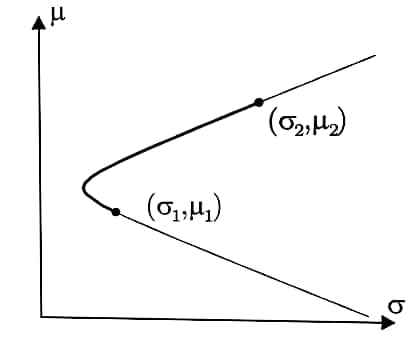
\includegraphics[width=10cm]{4.jpg}
    \caption{Hyperbola representing feasible portfolios with $-1<\rho_{12}<1$}
    \label{fig:SI}
\end{figure}

\begin{theorem}
    Suppose $\rho_{12}=1$ and $\sigma_{1} \neq \sigma_{2}$, then $\sigma_{V}=0$ if and only if \\$w_{1}=-\frac{\sigma_{2}}{\sigma_{1}-\sigma_{2}},w_{2}=\frac{\sigma_{1}}{\sigma_{1}-\sigma_{2}}$. This involves short selling as $w_{1}<0$ or $w_{2}<0.$
    \\Suppose $\rho_{12}=-1$, then $\sigma_{V}=0$ if and only if \\$w_{1}=\frac{\sigma_{2}}{\sigma_{1}+\sigma_{2}},w_{2}=\frac{\sigma_{1}}{\sigma_{1}+\sigma_{2}}$. This requires no short selling as $w_{1}>0$ or $w_{2}>0.$
\end{theorem}
\begin{proof}
    Let $\rho_{12}=1$ and $\sigma_{1} \neq \sigma_{2}$.
    \begin{align*}
        \sigma_{V}=0 &\iff \sqrt{w_{1}^2\sigma_{1}^{2}+w_{2}^2\sigma_{2}^{2}+2w_{1}w_{2}\sigma_{1}\sigma_{2}}=0\\
        &\iff w_{1}\sigma_{1}+w_{2}\sigma_{2}=0\\
        &\iff w_{1}=-\frac{\sigma_{2}}{\sigma_{1}-\sigma_{2}},w_{2}=\frac{\sigma_{1}}{\sigma_{1}-\sigma_{2}} &\{\text{Since } w_{1}+w_{2}=1\}
    \end{align*}
    Let $\rho_{12}=-1$.
    \begin{align*}
        \sigma_{V}=0 &\iff sqrt{w_{1}^2\sigma_{1}^{2}+w_{2}^2\sigma_{2}^{2}-2w_{1}w_{2}\sigma_{1}\sigma_{2}}=0\\
        &\iff w_{1}\sigma_{1}-w_{2}\sigma_{2}=0\\
        &\iff w_{1}=\frac{\sigma_{2}}{\sigma_{1}+\sigma_{2}},w_{2}=\frac{\sigma_{1}}{\sigma_{1}+\sigma_{2}} &\{\text{Since } w_{1}+w_{2}=1\}
    \end{align*}
\end{proof}
\begin{figure}[htp]
    \centering
    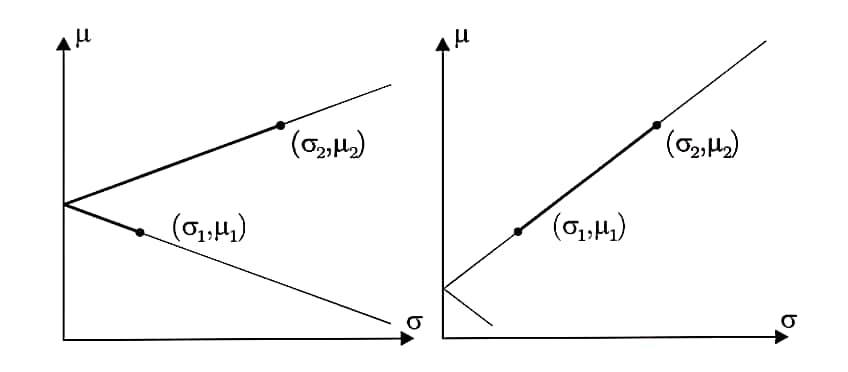
\includegraphics[width=15cm]{5.jpg}
    \caption{Typical portfolio lines with $\rho_{12}=$ -1 and 1}
    \label{fig:SI}
\end{figure}

\begin{theorem}
    Suppose that $\sigma_{1} \leq \sigma_{2}$. The following five cases are possible.
    \begin{enumerate}
        \item If $\rho_{12}=1$, then there is a feasible portfolio V with short selling such that $\sigma_{V}=0$ whenever $\sigma_{1}<\sigma_{2}$. Each portfolio V in the feasible set has the same $\sigma_{V}$ whenever $\sigma_{1}=\sigma_{2}$.
        \item If $\frac{\sigma_{1}}{\sigma_{2}}<\rho_{12}<1$, then there is a feasible portfolio V with short selling such that $\sigma_{V}=\sigma_{1}$, but for each portfolio without short selling $\sigma_{V} \geq \sigma_{1}$.
        \item If $\rho_{12}=\frac{\sigma_{1}}{\sigma_{2}}$, then $\sigma_{V} \geq \sigma_{1}$ for each feasible portfolio V.
        \item If $-1<\rho_{12}<\frac{\sigma_{1}}{\sigma_{2}}$, then there is a feasible portfolio V without short selling such that $\sigma_{V}<\sigma_{1}$.
        \item If $\rho_{12}=-1$, then there is a feasible portfolio V without short selling such that $\sigma_{V}=0$.
    \end{enumerate}
\end{theorem}
\begin{figure}[htp]
    \centering
    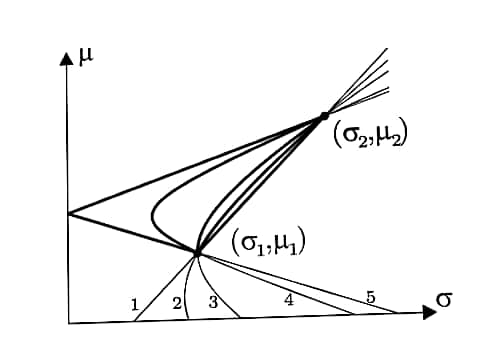
\includegraphics[width=12cm]{6.jpg}
    \caption{portfolio lines for various values of $\rho_{12}$}
    \label{fig:SI}
\end{figure}
\section{Several Securities}
\subsection{Risk and Expected Return of a Portfolio}
Let us consider a portfolio which is constructed from n different securities with the weight of each asset being $$w_{i}=\frac{x_{i}S_{i}(0)}{V(0)}, \hspace{10mm} i=1,\cdots,n,$$
where $x_{i}$ is the number of shares of type $i$ in the portfolio, $S_{i}(0)$ is the initial price of security $i$ and $V(0)$ is the initial amount invested in portfolio.
We introduce following notions \-
\begin{align*}
    \text{Weight vector } \mathbf{w}&=[\,\,w_{1}\,\,w_{2}\,\,\cdots\,\,w_{n}\,\,]\\
    \text{Unit vector } \mathbf{u}&=[\,\,1\,\,1\,\,\cdots\,\,1\,\,]\\
    \text{Expectation vector }    \mathbf{m}&=[\,\,\mu_{1}\,\,\mu_{2}\,\,\cdots\,\,\mu_{n}\,\,] \hspace{10mm} \text{where } \mu_{i}=\mathbb{E}(K_{i}) \,\, \forall i=1,\cdots,n\\
    \text{Covariance matrix } \mathbf{C}&=\left[
\begin{array}{ccc}
   c_{11} & \cdots & c_{1n} \\
   \vdots & \ddots & \vdots \\
   c_{n1} & \cdots & c_{nn} 
\end{array}
\right]\\ &\hspace{10mm} \text{where } c_{ij}=Cov(K_{i},K_{j}) \,\, \text{and } c_{ii}=\sigma_{i}^{2}=Var(K_{i}) \,\, \forall i,j=1,\cdots,n\\
\end{align*}
The condition of the sum of all weights being 1, can be written as \-
\begin{equation}
    1=\mathbf{wu}^{T}
\end{equation}
Assume that $det \, \mathbf{C} \neq 0 \Rightarrow \mathbf{C}^{-1}$ exists.
\\Return on portfolio V
\begin{equation}
    K_{V}=w_{1}K_{1}+w_{2}K_{2}+\cdots+w_{n}K_{n}
\end{equation}
\\Expected returns
\begin{equation}
    \mu_{V}=\mathbb{E}(K_{V})= \mathbf{wm}^{T}
\end{equation}
\\Varianvce
\begin{equation}
    \sigma_{V}^{2}=Var(K_{V})=\mathbf{wCw}^{T}
\end{equation}
$\{ \because Var(X)=Cov(X,X) \, \& Cov(\displaystyle \sum_{i=1}^{n} w_{i}K_{i}, \sum_{j=1}^{m} w_{j}K_{j}) = \sum_{i=1}^{n} \sum_{j=1}^{m} w_{i}w_{j}Cov(K_{i},K_{j})\}$

\subsection{Minimum Variance Portfolio}
The portfolio with the smallest variance among all feasible portfolios will be called the minimum variance portfolios or MVP. To find this, we need to solve,
\begin{equation}
    \text{Min }\sigma_{V}^2=\text{Min }\mathbf{wCw}^{T} \hspace{10mm} \text{subject to } \mathbf{wu}^{T}=1 \hspace{10mm} \text{for }\mathbf{w} \in \mathbb{R}^{n}.
\end{equation}

\begin{theorem}
    Let $det \, \mathbf{C} \neq 0$, then the MVP has weights $w_{MVP}=\frac{\mathbf{uC}^{-1}}{\mathbf{uC}^{-1}\mathbf{u}^{T}}$. 
\end{theorem}
\begin{proof}
Using Lagrange Multiplier Method, ($\lambda \Rightarrow$ Lagrange Multiplier)
$$F(\mathbf{w},\lambda)=\mathbf{wCw}^{T}-\lambda(\mathbf{wu}^{T}-1)$$
First order necessary condition gives, $\mathbf{2wC-\lambda u=0}$ or $\mathbf{w=\frac{\lambda}{2}uC}^{-1}$.
$$\Rightarrow \frac{\lambda}{2}\mathbf{uC}^{-1}\mathbf{u}^{T}=1$$
$$\Rightarrow \frac{\lambda}{2}=\frac{1}{\mathbf{uC}^{-1}\mathbf{u}^{T}}$$
$\{\because c_{ij} \geq 0 \Rightarrow C$ is SPD $\Rightarrow C^{-1}$ is also SPD $\Rightarrow \mathbf{uC}^{-1}\mathbf{u}^{T}>0\}$
$\\\{\because \sigma_{V}^{2}$ is bounded below by zero , so it must have a minimum $\}$
$$\Rightarrow w_{MVP}=\frac{\mathbf{uC}^{-1}}{\mathbf{uC}^{-1}\mathbf{u}^{T}}$$
\end{proof}
\subsection{Efficient Frontier}
\subsubsection{Dominating Security}
A security with expected return $\mu_{1}$ and standard deviation $\sigma_{1}$ is said to dominate another security with expected return $\mu_{2}$ and standard deviation $\sigma_{2}$ provided $\mu_{1}\geq\mu_{2}$ and $\sigma_{1}\leq\sigma_{2}$.
\subsubsection{Efficient Frontier}
A portfolio is called efficient if there is no other portfolio except itself, that dominates it. The subset of efficient portfolios among all feasible portfolios is called the efficient frontier. In order to determine the efficient frontier, we need to identify and eliminate the dominated portfolios.
\subsubsection{Minimum Variance Line}
The family of portfolio V, parameterised by $\mu \in \mathbb{R}$ such that $\mu_{V}=\mu$ and $\sigma_{V}^{2} \leq \sigma_{V'}^{2}$ for each portfolio V' with $\mu_{V'}=\mu$ is called the minimum variance line or MVL.

\begin{equation*}
    \text{Min }\sigma_{V}^2=\mathbf{wCw}^{T} \hspace{7mm} \text{subject to } \mathbf{wu}^{T}=1 \text{ and } \mathbf{wm}^{T}=\mu \hspace{7mm} \text{for }\mathbf{w} \in \mathbb{R}^{n} , \mu \in \mathbb{R}.
\end{equation*}

Using Lagrange Multiplier Method, ($\lambda_{1} , \lambda_{2} \Rightarrow$ Lagrange Multipliers)
$$G(\mathbf{w},\lambda_{1},\lambda_{2})=\mathbf{wCw}^{T}-\lambda_{1}(\mathbf{wm}^{T}-\mu)-\lambda_{2}(\mathbf{wu}^{T}-1)$$
First order necessary condition gives, $$\mathbf{2wC-\lambda_{1}m-\lambda_{2}u=0} \text{ or } \mathbf{w=\frac{1}{2}(\lambda_{1}m+\lambda_{2}u)C}^{-1}.$$
$$\Rightarrow \mathbf{\frac{1}{2}(\lambda_{1}m+\lambda_{2}u)C}^{-1}\mathbf{m}^{T}=\mu \text{ and } \mathbf{\frac{1}{2}(\lambda_{1}m+\lambda_{2}u)C}^{-1}\mathbf{u}^{T}=1$$
\begin{equation}
  Define M=\begin{bmatrix}
\mathbf{mC^{-1}m^{T}} & \mathbf{uC^{-1}m^{T}}\\
\mathbf{mC^{-1}u^{T}} & \mathbf{uC^{-1}u^{T}}
\end{bmatrix}=\begin{bmatrix}
p & q\\
r & s 
\end{bmatrix} \hspace{10mm} \text{(say)}  
\end{equation}

$$ \Rightarrow \begin{bmatrix}
\lambda_{1}\\
\lambda_{2}
\end{bmatrix}=2 M^{-1} 
\begin{bmatrix}
\mu\\
1
\end{bmatrix}$$
$$\Rightarrow w_{MVL}=\mu\mathbf{\frac{(smC^{-1}-ruC^{-1})}{(ps-qr)}}+\mathbf{\frac{(puC^{-1}-qmC^{-1})}{(ps-qr)}} = \mu\mathbf{a+b} \text{ where } \mathbf{a},\mathbf{b} \in \mathbb{R}^{n}$$
This can be summarised in the following theorem.
\newpage
\begin{theorem}
    Let det $\mathbf{C} \neq 0 \text{ and } \mathbf{m , u}$ are linearly independent vectors, then the weight vector $\mathbf{w}$ represents a portfolio V on the minimum variance line if and only if $$\Rightarrow w_{MVL}=\mu\mathbf{\frac{(smC^{-1}-ruC^{-1})}{(ps-qr)}}+\mathbf{\frac{(puC^{-1}-qmC^{-1})}{(ps-qr)}}$$ with $\mu = \mu_{V}$ and notations of (3.18).
\end{theorem}

\begin{theorem} [Two Fund Theorem]
    Under the assumptions of the previous theorem, let $\mathbf{w_{1}}$ and $\mathbf{w_{2}}$ be the weights of any two portfolios $V_{1},V_{2}$ on the minimum variance line with different expected returns $\mu_{V_{1}}\neq\mu_{V_{2}}$. Then each portfolio V on the minimum variance line can be obtained as a linear combination of these two, i.e., $$\mathbf{w}=\alpha\mathbf{w_{1}}+(1-\alpha)\mathbf{w_{2}} \hspace{10mm} \text{ for some } \alpha \in \mathbb{R}$$
\end{theorem}
\begin{proof}
Define $\alpha = \frac{\mu_{V}-\mu_{V_{2}}}{\mu_{V_{1}}-\mu_{V_{2}}}$
\begin{align*}
        \alpha\mathbf{w_{1}}+(1-\alpha)\mathbf{w_{2}} &= \alpha (\mu_{V_{1}}\mathbf{a+b}) + (1-\alpha)(\mu_{V_{2}}\mathbf{a+b}) \\
        &= (\alpha \mu_{V_{1}} + (1-\alpha)\mu_{V_{2}})\mathbf{a+b} \\
        &= \mu_{V}\mathbf{a+b} = \mathbf{w} \\
\end{align*}
\end{proof}
%\subsubsection{Implication}
%Any portfolio on the MVL can be realised by splitting the available investment amount between just two different portfolios instead of investing in individual assets.
Following pdf contains the practical implementation of the theory described in this chapter.
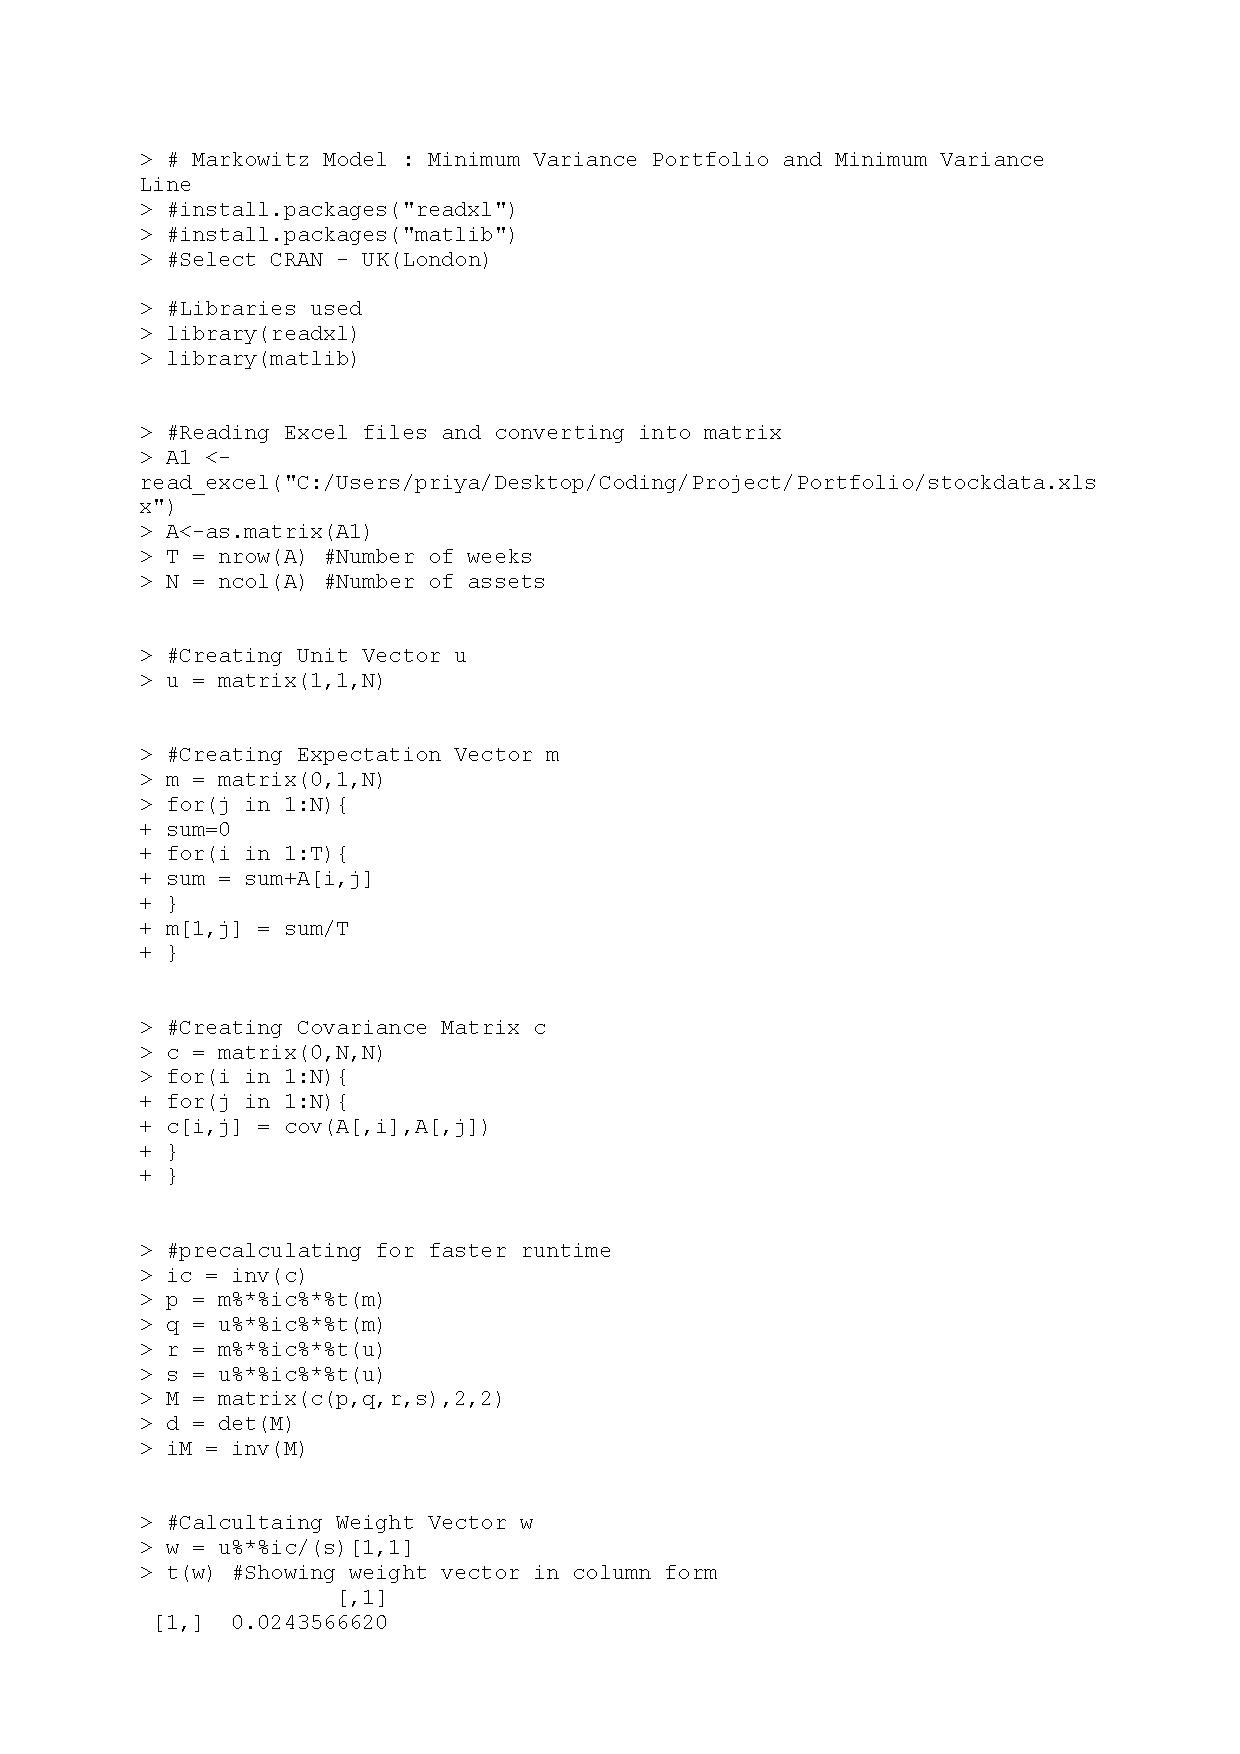
\includepdf[pages=-]{output_text.pdf}